% =====================================================================
% main.tex — SOCC 2026 CAMERA-READY (de-anonymized)
%
% TLG-mapped BNN tile in a fully-digital sky130 SoC built with the
% open-flow (LibreLane + OpenRAM + PicoRV32). 6-page IEEE conference
% format, ~3,500 words body, 4 figures, 2 tables, ~28 references.
%
% The review copy is frozen under ../paper/. Figures are shared from
% ../paper/figures (see \graphicspath); tables/ and refs.bib are
% snapshots that may diverge with reviewer-driven revisions.
%
% Build:  make           (pdflatex + bibtex + pdflatex x2)
% Clean:  make clean
% Pre-upload checklist: README.md
% =====================================================================

\documentclass[conference]{IEEEtran}
% Required for the full-width \IEEEpubid copyright box below.
\IEEEoverridecommandlockouts

\usepackage{cite}
\usepackage{amsmath,amssymb,amsfonts}
\usepackage{graphicx}
\usepackage{booktabs}
\usepackage{textcomp}
\usepackage{xcolor}
\usepackage{url}
\usepackage{placeins}

% Figures stay single-sourced in the review tree; build them with
% `make -C ../paper figures`.
\graphicspath{{../paper/figures/}}

% XNOR operator (binary-inner-product idiom under {-1,+1} -> {0,1}
% encoding) — used in Sections I and III-B.
\newcommand{\xnor}{\mathbin{\overline{\oplus}}}
\hyphenation{Open-RAM Wish-bone}

\begin{document}

% ---------------------------------------------------------------------
% TODO(camera-ready): paste the copyright/ISBN line from the SOCC
% acceptance e-mail into the \IEEEpubid below and uncomment it.
% Placement verified: with \IEEEoverridecommandlockouts above and the
% \IEEEpubid here (immediately after \begin{document}), the notice sets
% at the foot of page 1 column 1 without colliding with column 2, and
% the paper still fits 6 pages. \IEEEpubidadjcol is not needed.
% ---------------------------------------------------------------------
% \IEEEpubid{\makebox[\columnwidth]{979-8-XXXX-XXXX-X/26/\$31.00~\copyright2026 IEEE \hfill}
%   \hspace{\columnsep}\makebox[\columnwidth]{}}

% ---------------------------------------------------------------------
% Title and de-anonymized author block (camera-ready).
% TODO(camera-ready): confirm author list, order, and e-mail addresses;
% affiliations must match the signed IEEE copyright form.
% ---------------------------------------------------------------------
\title{TINKER: A Fully-Digital Threshold-Logic-Mapped\\
  BNN Inference SoC}

\author{\IEEEauthorblockN{Abdullah Sahruri and Martin Margala}
  \IEEEauthorblockA{\textit{School of Computing and Informatics},
    \textit{University of Louisiana at Lafayette}, Lafayette, LA, USA\\
    \{abdullah.sahruri1, martin.margala\}@louisiana.edu}}

\maketitle

% ---------------------------------------------------------------------
% Abstract — fill last (Stage 7).
% ---------------------------------------------------------------------
\begin{abstract}
  This paper presents TINKER, a complete open-flow RISC-V inference
  SoC that integrates a sixteen-neuron binary neural network (BNN)
  tile with a PicoRV32 RV32I core, a Wishbone B4 fabric, and
  OpenRAM-based instruction/data memories in SkyWater sky130A. The
  tile implements XNOR/popcount/threshold neuron behavior through a
  fully digital threshold-logic mapping: the 64-bit threshold
  function is decomposed into chunked LUT sub-popcounts, an adder
  tree, and a comparator, all synthesized into ordinary standard
  cells. This avoids analog, current-mode, memristor, or flash
  primitives while preserving a portable RTL-to-GDS implementation
  path. TINKER runs a grouped 14\(\times\)14 MNIST BNN through five
  software-scheduled tile evaluations and reaches 85.60\,\%
  accuracy on the full 10\,000-image test set, with a 95\,\%
  Wilson confidence interval of [84.90\,\%, 86.27\,\%]. Post-P\&R
  activity-aware evaluation reports 47.21\,mW and
  8.06\,\textmu J/inference; the TLG tile accounts for 24.3\,\% of
  total SoC power, the largest active datapath bucket after the
  memory subsystem is implemented with OpenRAM macros. Physical
  verification is clean on KLayout DRC, Netgen LVS, KLayout XOR,
  and antenna. Timing closes at the headline TT corner; slow-corner
  macro timing is limited by OpenRAM's single-corner Liberty model.
\end{abstract}

\begin{IEEEkeywords}
  binary neural networks, threshold logic, system-on-chip, RISC-V,
  open-source EDA.
\end{IEEEkeywords}

\section{Introduction}
\label{sec:intro}



Binary neural networks (BNNs) are attractive for small inference
SoCs because multiplication collapses to bitwise XNOR and
population count. The remaining question is not whether a BNN
inner product can be synthesized, but whether a threshold-logic
view of that inner product can be mapped into a complete,
portable SoC implementation. Classical threshold logic fires when
a weighted sum crosses a programmed threshold~\cite{beiu2003vlsi},
yet prior silicon demonstrations commonly rely on fabrication-bound
primitives such as current-mode summation~\cite{beiu2003differential},
memristors~\cite{papandroulidakis2019memristor}, or embedded
flash threshold devices~\cite{wagle2020tulip}. Fig.~\ref{fig:conventional}
illustrates the conventional view: panel (a) is the abstract
weighted-sum threshold neuron, and panel (b) is a representative
capacitive realization that ties the threshold function to a
specific analog primitive. Those approaches are useful
architectural comparators, but they do not answer whether
threshold-logic-mapped BNN compute can live inside an ordinary
digital RTL-to-GDS flow.
\begin{figure}[!t]
  \centering
  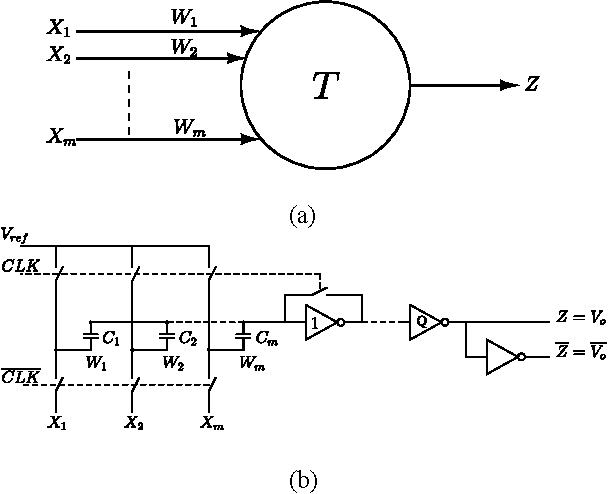
\includegraphics[width=\columnwidth]{conventional3.pdf}
  \caption{Conventional threshold-logic neuron: (a) abstract
    weighted-sum-threshold model and (b) a representative capacitive
    realization~\cite{ozdemir1996capacitive} with charge redistribution onto weighted
    capacitors $C_i$ followed by a clocked inverter chain. TINKER
    replaces this fabrication-bound primitive with a fully digital
    chunked-LUT mapping (Section~\ref{sec:arch:tile}).}
  \label{fig:conventional}
\end{figure}
TINKER addresses this question with a fully digital
threshold-logic-mapped BNN tile integrated into an open-flow
RISC-V SoC. Each neuron computes XNOR/popcount/threshold behavior,
but the 64-bit threshold function is implemented by a chunked-LUT
decomposition: fixed-size LUT sub-popcounts feed an adder tree and
a comparator, all synthesized into \texttt{sky130\_fd\_sc\_hd}
standard cells. The tile is attached to a PicoRV32~\cite{wolf2015picorv32}
RV32I core over a Wishbone B4 fabric with OpenRAM
IMEM/DMEM macros~\cite{guthaus2016openram}. Firmware schedules a grouped
14\(\times\)14 MNIST BNN through five sequential tile evaluations.
This combination makes the work a hardware/software co-design and
SoC-integration study, not an isolated accelerator macro.

The paper makes three contributions:
\begin{itemize}
  \item a standard-cell chunked-LUT threshold-logic decomposition
        for BNN neurons, avoiding analog, current-mode, memristor, or
        flash primitives;
  \item a complete PicoRV32/Wishbone B4/OpenRAM inference SoC in
        the sky130A open RTL-to-GDS flow; and
  \item post-P\&R activity-aware evaluation showing 85.60\,\%
        MNIST accuracy, 8.06\,\textmu J/inference, and a TLG tile that
        accounts for 24.3\,\% of total SoC power, the largest active
        datapath bucket once register-file memories are replaced by
        OpenRAM macros.
\end{itemize}

\section{Background and Related Work}
\label{sec:background}

We organize prior work along three axes: (i)~the device primitive
used to realize the threshold function, (ii)~the scope of the
demonstration (gate, accelerator IP, or full SoC), and (iii)~the
openness of the implementation flow. TINKER occupies a specific
cell in this space: a digital standard-cell primitive realized
through chunked-LUT decomposition, integrated as a software-orchestrated
SoC, in a fully open RTL-to-GDS flow.

\subsection{Threshold-logic primitives}
Most prior silicon TLG demonstrations bind the threshold function
to a fabrication-specific primitive. Differential and current-mode
designs realize the weighted sum electrically through summed
branch currents~\cite{beiu2003differential}, with compact gates
but bias- and matching-dependent behavior that does not survive
process migration. Capacitive realizations~\cite{ozdemir1996capacitive}
encode weights as capacitor ratios with a precharge phase, with
high fan-in variants adding offset
compensation~\cite{sahruri2024hictl} or key-driven charge
recycling for logic locking~\cite{sahruri2025tlglock}.
Memristor-based TLGs~\cite{papandroulidakis2019memristor} use
non-volatile resistance for both weight storage and analog
summation, gaining device-level density at the cost of integration
with mainstream digital flows. TULIP~\cite{wagle2020tulip} is the
closest threshold-logic ASIC comparator: it realizes a configurable
BNN as a network of programmable threshold-logic standard cells
whose threshold compare uses embedded flash, establishing the
TLG-network view of BNN inference at accelerator scope but
inheriting the process-portability limits of flash and reporting
as a macro rather than a software-orchestrated SoC. The broader
standard-cell threshold-logic synthesis
literature~\cite{beiu2003vlsi} shares TINKER's mapping style but
targets gate- and netlist-level synthesis; the contribution here
is one of scope, not new gate-level theory.

\subsection{Digital BNN accelerators and open-flow SoCs}
Digital BNN accelerators set the energy frontier for the
XNOR-popcount-threshold datapath in commercial flows.
YodaNN~\cite{andri2018yodann}, XNE~\cite{conti2018xnor}, and
ChewBaccaNN~\cite{andri2021chewbaccann} target 65--22\,nm
processes and report sub-microjoule per inference;
FINN~\cite{umuroglu2017finn} demonstrates the same datapath in
an FPGA dataflow framework. Closest to the mapping used here,
TLG2LUT6~\cite{sahruri2026tlg2lut6} folds binary weights and
thresholds into LUT6 initialization strings, but is tied to a
vendor fabric; the decomposition here targets standard cells and
is carried to GDS inside a complete SoC. None of these targets a fully
open-source RTL-to-GDS flow, and most report accelerator IP
rather than a software-orchestrated SoC. The closest open-flow
sky130 comparator is OpenSpike~\cite{modaresi2023openspike},
which combines PicoRV32 and OpenRAM but targets a spiking
network and does not address threshold-logic decomposition. The
contribution here is therefore not raw efficiency at advanced
nodes; it is an open, portable demonstration that a
threshold-logic decomposition survives integration into a
complete RISC-V SoC under software control. The chunked-LUT
mapping introduced in Section~\ref{sec:arch:tile} is the
mechanism by which TINKER meets that constraint within an
ordinary digital RTL-to-GDS flow.

\section{SoC Architecture}
\label{sec:arch}

\begin{figure}[t]
  \centering
  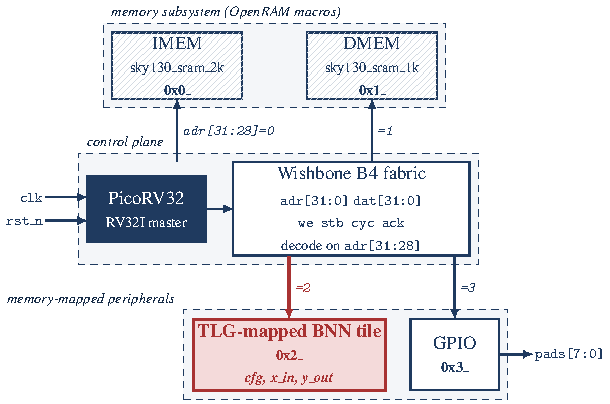
\includegraphics[width=\columnwidth]{fig1_soc_block.pdf}
  \caption{SoC architecture block diagram: PicoRV32 master,
    Wishbone B4, OpenRAM IMEM/DMEM, TLG-mapped tile, and GPIO.}
  \label{fig:soc-block}
\end{figure}

\begin{figure*}[t]
  \centering
  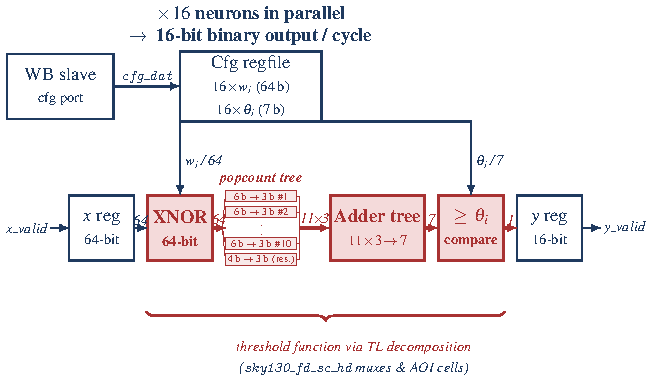
\includegraphics[width=0.68\textwidth]{fig2_tile_microarch.pdf}
  \caption{TLG-mapped BNN tile microarchitecture. Sixteen
    XNOR-popcount-threshold neurons share the registered input,
    use eleven chunk-LUT sub-popcounts per neuron, and produce a
    16-bit output vector.}
  \label{fig:tile-microarch}
\end{figure*}

\subsection{System overview}
\label{sec:arch:overview}

TINKER is a single-clock RV32I system that hosts and orchestrates
the TLG-mapped tile under software control. A
PicoRV32 core~\cite{wolf2015picorv32} acts as the lone Wishbone B4 classic
master and drives a single-cycle bus with 32-bit address and
32-bit data; address decode on \texttt{adr[31:28]} dispatches to
one of four word-aligned slaves: IMEM at
\texttt{0x0000\_0000}, DMEM at \texttt{0x1000\_0000}, the tile
peripheral at \texttt{0x2000\_0000}, and a sim-observability
GPIO at \texttt{0x3000\_0000}. Reset is asynchronously asserted
and synchronously deasserted through a two-stage flop chain;
firmware boots bare-metal from \texttt{PROGADDR\_RESET\,=\,0}.
A single-master, four-slave decode is sufficient for the polled
inference handshake. The system clock is nominally 100\,MHz,
matching the standalone tile constraint. Fig.~\ref{fig:soc-block}
shows the block diagram.

\subsection{Threshold-logic decomposition and tile microarchitecture}
\label{sec:arch:tile}

\paragraph{Neuron function} Each tile neuron computes the
binary inner product
\(y_i = \mathbf{1}\!\left[\,\mathrm{popcount}\!\left(x \xnor w_i\right) \ge \theta_i\,\right]\),
with \(x \in \{-1,+1\}^{64}\) and per-neuron 64-bit weight \(w_i\)
and 7-bit threshold \(\theta_i\). This realizes threshold-function
behavior without instantiating a literal high-fanin physical
threshold gate. Sixteen neurons share the registered input and
produce a 16-bit output vector per evaluation, with two-cycle
latency.
Fig.~\ref{fig:tile-microarch} shows the tile datapath and
configuration path.

\begin{figure}[t]
  \centering
  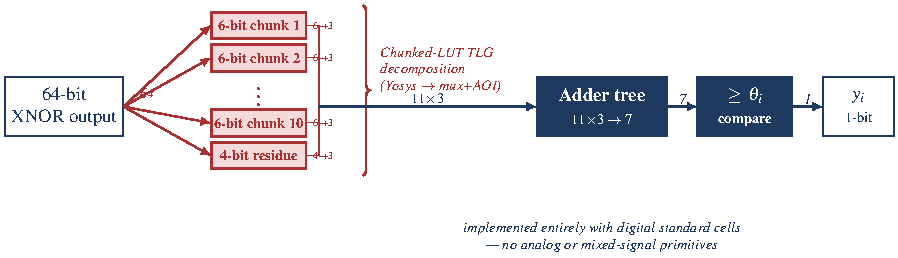
\includegraphics[width=\columnwidth]{fig_tlg_decomp.pdf}
  \caption{Chunked-LUT decomposition of the 64-bit threshold
    function. The XNOR output partitions into ten 6-bit chunks and
    one 4-bit residue; each sub-popcount is synthesized into
    \texttt{sky130\_fd\_sc\_hd} logic. The subcounts feed an adder
    tree and threshold comparator.}
  \label{fig:tlg-decomp}
\end{figure}

\paragraph{Chunked-LUT decomposition} The decomposition recasts
the 64-input threshold function as a small adder-tree of population
counts over fixed-size chunks. The 64-bit XNOR output is partitioned
into eleven chunks: ten 6-bit chunks plus one 4-bit residue.
Each 6-bit chunk's population count is a small Boolean function
($6 \to 3$) that Yosys synthesises into a network of
\texttt{sky130\_fd\_sc\_hd} multiplexers and AOI cells; the 4-bit
residue ($4 \to 3$) is similarly decomposed. The eleven 3-bit
subcounts feed a conventional width-7 adder tree, and the 7-bit
sum is compared against \(\theta_i\) by a standard magnitude
comparator. Fig.~\ref{fig:tlg-decomp} visualises the decomposition.
The chunked approach bounds fanin and avoids a fabrication-specific
summation primitive. The 6-bit chunk size matches
\texttt{sky130\_fd\_sc\_hd}'s mux/AOI cost: large enough that
the eleven-way partitioning overhead is acceptable, small enough
that each chunk LUT fits comfortably as a combinational cell
network.

\paragraph{Programmability} The configuration regfile holds 16 weight words (64-bit)
and 16 thresholds (7-bit), addressed through a 6-bit
\texttt{cfg\_addr}; weights are loaded once per network and the cfg
port carries traffic only at boot. An \texttt{x\_valid} strobe
latches the input register and starts the two-cycle pipeline;
\texttt{y\_valid} pulses on the cycle the output leaves.

\subsection{Tile wrapper and inference handshake}
\label{sec:arch:wrapper}

The Wishbone-to-tile bridge \texttt{wb\_tile\_wrapper} occupies a
512-byte slave window and exposes the tile's cfg port and
\(x_\text{in}/y_\text{out}\) handshake as memory-mapped registers.
Weights and inputs are committed by two-phase 32-bit writes
(\texttt{LO} then \texttt{HI}), with the \texttt{HI} write
assembling the 64-bit value and pulsing the corresponding strobe;
thresholds are atomic single-word writes. Firmware polls
\texttt{STATUS.BUSY} until clear, reads \texttt{YOUT}, and writes
\texttt{CTRL.CLR\_DONE} to arm the next inference. Writes to
weight, threshold, or input registers while \texttt{BUSY\,=\,1}
are silently dropped: the bus access acks normally but no shadow
is updated, causing a misbehaving program to hang visibly rather
than corrupt an in-flight evaluation. This is a deliberate
testability choice: a silently corrupted inference is a far worse
failure mode than an observably hung firmware loop. The wrapper
carries roughly 1.3\,K flops, $\sim$700 of them purely for read-back of
every writable register.

The memory subsystem instantiates pre-hardened OpenRAM~\cite{guthaus2016openram}
1RW1R macros: 2\,KB for IMEM and 1\,KB for DMEM. A small Wishbone
FSM wraps each macro and inserts one wait state on reads. The
motivation for OpenRAM macros over a register-file baseline is
power; the system-level consequence is detailed in
Section~\ref{sec:eval:power}.

\section{Workload Mapping and Deployment}
\label{sec:workload}

The deployed network is a grouped binary MLP over a
14\,\(\times\)\,14 input. After a 2\,\(\times\)\,2 average pool and a
per-quadrant median binarisation, four parallel branches each map a
49-bit quadrant to 16 hidden bits in one tile evaluation; the four
16-bit outputs concatenate into a 64-bit hidden vector that the same
tile maps to ten output logits in a fifth evaluation. Grouping
(rather than full $196 \to 64$ connectivity) is a hardware-shape
choice: each branch fits one tile-evaluation fanin, so the entire
network maps onto the SoC without changing tile or wrapper RTL.
The accuracy cost of grouping was bounded before deployment with a
float-precision proxy: trained on the same data with the same
preprocessing, a grouped $4 \times (49 \to 16)$ model trails an
unconstrained $196 \to 64$ model by 0.87\,pp. That gap is the same
order as the deployed network's own experimental spread---0.74\,pp
across the three training seeds, and a 0.69\,pp half-width on the
95\,\% Wilson confidence interval---and an order below the accuracy
given up to binarisation itself.
Per-image inference therefore costs four hidden-layer batches plus
one output-layer batch, which the PicoRV32 firmware schedules
sequentially against the cfg-write/poll/read protocol of
Section~\ref{sec:arch:wrapper}, totalling 17\,068 cycles or
170.7\,\textmu s at 100\,MHz. The bare-metal firmware compiles to
roughly 1.5\,KB of RV32I and shares the IMEM with the binary weights;
per-image input bits are preloaded into DMEM by the testbench at
simulation time zero. A vectorised Python integer model serves as
the deployment golden, folding the trained batch-norm parameters into
per-neuron thresholds via
$t_i = \lceil (49 + \mathrm{sgn}(\gamma_i)\,\mu_i - \beta_i\sigma_i/|\gamma_i|)/2 \rceil$;
SoC RTL simulation matches this golden on all sixteen verification
images. Weights are trained off-chip with
binary-weight gradient descent~\cite{courbariaux2015binaryconnect} and a hard-tanh
straight-through estimator~\cite{hubara2016bnn} on a OneCycleLR
schedule~\cite{smith2017superconvergence}.

\section{Implementation}
\label{sec:impl}

\subsection{Open-flow toolchain}
\label{sec:impl:flow}

The SoC is implemented through the LibreLane 3.0.3 RTL-to-GDSII
flow~\cite{librelane2025} on the SkyWater sky130A open-source PDK.
Yosys synthesises the design against the
\texttt{sky130\_fd\_sc\_hd} standard-cell library;
OpenROAD~\cite{ajayi2019openroad} drives floorplanning, placement, clock-tree
synthesis, routing, and antenna repair; Magic and KLayout perform GDS
streamout and DRC; Netgen performs LVS. The OpenRAM IMEM and DMEM
macros occupy 683\(\times\)417\,\textmu m and
480\(\times\)398\,\textmu m, respectively, and are manually placed in
a 1\,500\(\times\)1\,500\,\textmu m absolute floorplan with PDN
hookups to the sky130 dual rail.
Macro integration required iteration on placement constraints, an
OpenSTA blackbox stub for the behavioural macro views, and removal of
the wrapper-level \texttt{keep\_hierarchy} attributes to satisfy
LibreLane's flat-macro convention. The full RTL-to-GDSII pipeline
uses one flow configuration for multi-corner STA, physical
verification, and activity-aware power decomposition.

\subsection{Sign-off methodology}
\label{sec:impl:signoff}
\begin{figure}[t]
  \centering
  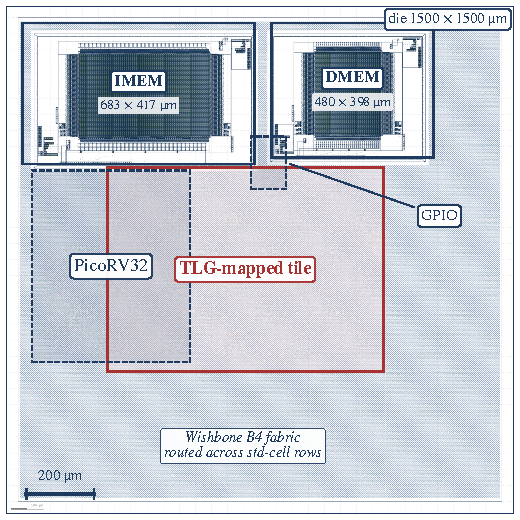
\includegraphics[width=\columnwidth]{fig3_layout.pdf}
  \caption{Post-P\&R floorplan of the open-flow BNN inference SoC on
    sky130A (1.5\,$\times$\,1.5\,mm$^2$ die). The IMEM and DMEM OpenRAM
    macros sit in the upper region; module footprints for the
    TLG-mapped tile, PicoRV32 core, Wishbone B4 fabric, and GPIO are
    extracted from the placed instance bounding boxes.}
  \label{fig:layout}
\end{figure}

Fig.~\ref{fig:layout} shows the post-P\&R floorplan, with the IMEM
and DMEM macros along the upper edge of the die and the std-cell logic
below. Multi-corner static timing was run across nine corners covering
the three sky130 process points (TT, FF, SS), three temperatures
($-40$\,\textdegree{}C, 25\,\textdegree{}C, 100\,\textdegree{}C), and
three supply voltages (1.60\,V, 1.80\,V, 1.95\,V). At the headline
\texttt{nom\_tt\_025C\_1v80} corner the design closes with
$+0.51$\,ns setup slack and $+0.37$\,ns hold slack; hold timing is
clean across all nine corners. Slow-corner setup violations at
\texttt{nom\_ss\_100C\_1v60} are an attribute of the OpenRAM macros'
single TT-corner Liberty, a documented LibreLane 3.x limitation
discussed in Section~\ref{sec:discussion}, not a design defect.
Physical verification is clean on KLayout DRC, Netgen LVS, KLayout
XOR, and antenna: respectively 0 errors, 0 errors, 0 differences,
and 0 violating nets/pins. The Magic DRC flags inside hardened SRAM
macro footprints are excluded from this claim because they are a
known sky130 macro-view issue.

\section{Evaluation}
\label{sec:eval}

\subsection{Functional verification}
\label{sec:eval:verif}

The deployed network is exercised through four verification gates,
summarised in Table~\ref{tab:verification}. The vectorised Python
integer model is treated as the deployment golden, since its
arithmetic is exact in the same fixed-width integer
domain as the on-chip XNOR-popcount; the trained PyTorch model is a
training-time proxy whose floating-point activations may differ near
batch-norm thresholds. The 16-image verification set is the first
16 images of the MNIST test split, used as a fast bit-exact check; the
full 10\,000-image test set is covered by the integer-golden gate.
PyTorch and the integer golden agree on 15 of these 16 images. The
single mismatch lies on a folded-batch-norm activation
boundary near zero and is the expected behaviour of the integer
quantisation, not a bug. The post-P\&R SoC RTL simulation then matches
the integer golden bit-exact on all sixteen images. On the full
10\,000-image MNIST test set~\cite{lecun1998gradient}, the same network reaches
85.60\,\% accuracy (8\,560 correct), with a 95\,\% Wilson confidence interval of
\([84.90\,\%,\,86.27\,\%]\); per-class accuracy ranges from 95.2\,\%
on digit~1 to 75.1\,\% on digit~5.
% Table I — Functional verification summary (4 gates).
% Numbers locked from PHASE4_5_NOTES.md §6 and PHASE3_5_NOTES.md §3.
\begin{table}[t]
  \centering
  \caption{Functional verification summary.}
  \label{tab:verification}
  \renewcommand{\arraystretch}{1.15}
  \begin{tabular}{@{}>{\raggedright\arraybackslash}p{0.36\columnwidth}>{\raggedright\arraybackslash}p{0.27\columnwidth}>{\raggedright\arraybackslash}p{0.27\columnwidth}@{}}
    \toprule
    \textbf{Gate} & \textbf{Reference} & \textbf{Result} \\
    \midrule
    PyTorch $\leftrightarrow$ integer golden & integer model & 15/16 (1 boundary) \\
    SoC sim $\leftrightarrow$ integer golden & RTL simulation & 16/16 PASS         \\
    Full MNIST 10\,K eval                    & vectorized integer model    & 85.60\,\% [84.90, 86.27] \\
    DRC / LVS / XOR / antenna               & KLayout, Netgen             & 0 / 0 / 0 / 0      \\
    \bottomrule
  \end{tabular}
\end{table}


\subsection{Activity-aware power decomposition}
\label{sec:eval:power}

Activity-aware power is reported at the headline
\texttt{max\_ff\_n40C\_1v95} corner. The full sixteen-image inference
testbench is replayed against the post-P\&R netlist, the chip-pin VCD
is annotated through OpenSTA's \texttt{read\_vcd}, supplemented with
forty-seven named-net activities for the major interior wires, and
\texttt{report\_power} is decomposed into per-instance buckets by
a bucketization pass. Total post-P\&R power is
47.21\,mW. Fig.~\ref{fig:power_breakdown} shows the hierarchical
decomposition. The clock tree is the largest single contributor at
15.10\,mW (32.0\,\%). The TLG-mapped tile is the largest active
datapath bucket at 11.47\,mW (24.3\,\%); the PicoRV32 core draws
7.71\,mW (16.3\,\%); the IMEM and DMEM macros draw 5.56\,mW
(11.8\,\%) and 3.85\,mW (8.2\,\%) respectively; shared logic and the
GPIO slave account for 1.24\,mW (2.6\,\%) and 0.30\,mW (0.6\,\%).
\begin{figure}[t]
  \centering
  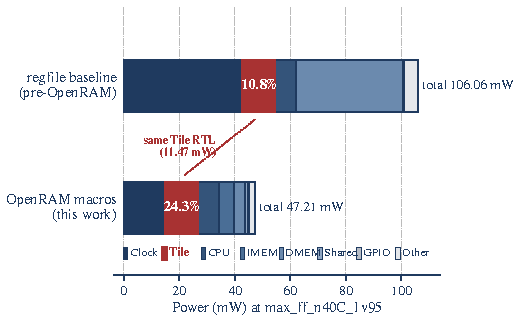
\includegraphics[width=\columnwidth]{fig4_power_breakdown.pdf}
  \caption{Hierarchical activity-aware power decomposition of the
    open-flow SoC at \texttt{max\_ff\_n40C\_1v95} (total 47.21\,mW).
    The TLG-mapped tile is the largest active datapath bucket once
    the OpenRAM macros remove register-file dominance from the
    memory subsystem.}
  \label{fig:power_breakdown}
\end{figure}

The actionable insight is the change in the tile's share of the
budget. With the register-file IMEM/DMEM of the Phase~3 baseline, the
same tile RTL (byte-identical post-flatten netlist) contributed
11.47\,mW of an SoC total of 106.06\,mW, or 10.81\,\%. Replacing the
register files with OpenRAM macros drops the system total to
47.21\,mW while leaving the tile bucket unchanged, lifting the tile's
share to 24.29\,\% and dropping the memory subsystem's combined share
from 36.4\,\% to 19.9\,\%. This share is not, by itself, an
efficiency claim; it is architectural evidence that compute remains
load-bearing at SoC scale after the memory subsystem is converted
from register files to OpenRAM macros.

\subsection{Energy and throughput}
\label{sec:eval:energy}

At the same \texttt{max\_ff} corner, the SoC executes 17\,068 cycles
per image, i.e.\ 170.7\,\textmu s and \textbf{8.06\,\textmu J per
  inference} at 100\,MHz. This corresponds to \textbf{124\,113
  inferences/J} and a sustained throughput of 5\,860\,inf/s under
continuous polling. The companion \texttt{nom\_tt\_025C\_1v80} corner
is slightly more efficient at an estimated 7.09\,\textmu J/image and
141\,044\,inf/J. Compared with the Phase~3 7\,\(\times\)\,7
deployment on the same SoC, the grouped 14\,\(\times\)\,14 network
gains $+14.48$\,pp of accuracy at $+1.0\,\%$ energy overhead per
image: the post-P\&R netlist, sign-off artefacts, and clock are
byte-identical, and only the firmware DMEM layout (8 vs 2 words/image)
and the binary weight image change between the two deployments. The
accuracy-per-microjoule figure of merit therefore rises from
8.91\,pp/\textmu J to 10.62\,pp/\textmu J, a 19.2\,\% improvement at
unchanged silicon.

\subsection{Tile ablation}
\label{sec:eval:ablation}

A same-flow standalone tile ablation compares the proposed
chunked-LUT TLG tile with a conventional synthesized
XNOR-popcount-comparator tile generated by the same scripts and run
through the same LibreLane tile flow. Table~\ref{tab:tlg-ablation}
shows the loadable variants, which include the programmable weight
and threshold register file needed by the SoC. The TLG mapping is
slightly larger and slower in this standalone flow, but reports
lower default-activity power. Because this ablation is tile-level
and uses OpenSTA default activity, the SoC-level claims in this
paper rely on the measured integrated TLG design rather than on a
projected replacement tile.
\begin{table}[t]
  \centering
  \caption{Same-flow standalone tile ablation. Both loadable variants use
  the same LibreLane tile flow, SDC, and 100\,MHz target; only the neuron
  RTL differs. Power is default-activity OpenSTA at the nominal corner.}
  \label{tab:tlg-ablation}
  \renewcommand{\arraystretch}{1.08}
  \begin{tabular}{@{}lcc@{}}
    \toprule
    \textbf{Metric} & \textbf{Chunked-LUT TLG} & \textbf{Adder-tree} \\
    \midrule
    Cells & 22\,125 & 21\,464 \\
    Area (\textmu m$^2$) & 320\,367 & 305\,300 \\
    Slow Fmax (MHz) & 73.81 & 77.51 \\
    Power (\textmu W) & 64\,566 & 167\,858 \\
    \bottomrule
  \end{tabular}
\end{table}


\subsection{Comparison with prior BNN ASICs}
\label{sec:eval:comparison}
% Table II — Comparison vs prior digital BNN/threshold-logic ASICs and
% the closest open-flow neural-inference comparator. Numeric cells for
% cited rows are populated from the cited papers' canonical PPA tables;
% see comments above each row for the verifying source.
\begin{table}[!t]
  \centering
  \caption{BNN/threshold-logic accelerator positioning. Designs differ in
  node, network, voltage, and reporting scope; the table is not a direct
  efficiency ranking. \textsuperscript{$\dagger$}~inherited training-method
  accuracy; \textsuperscript{$\ddagger$}~core dynamic energy only.}
  \label{tab:comparison}
  \scriptsize
  \renewcommand{\arraystretch}{1.15}
  \setlength{\tabcolsep}{3pt}
  \begin{tabular}{@{}llllll@{}}
    \toprule
    \textbf{Ref.} & \textbf{Tech.} & \textbf{Network} & \textbf{Acc.} & \textbf{E/inf.} & \textbf{Area} \\
    \midrule
    \cite{conti2018xnor}          & 22\,nm        & ResNet-18 IN     & 51.2\,\%               & 1\,450\,\textmu J               & 2.32\,mm$^2$ \\
    \cite{andri2018yodann}       & UMC 65\,nm    & AlexNet IN       & $\sim$56\,\%$^\dagger$ & 352\,\textmu J                  & 1.9\,mm$^2$  \\
    \cite{wagle2020tulip}            & 40\,nm        & BinaryNet C10    & 89.85\,\%$^\dagger$    & 184\,\textmu J                  & 1.8\,mm$^2$  \\
    \cite{andri2021chewbaccann}  & GF 22\,nm FDX & VGG-like C10     & 86.8\,\%               & 1.3\,\textmu J                  & 0.7\,mm$^2$  \\
    \cite{modaresi2023openspike}        & sky130        & 1024-1024-10 SNN & 99.12\,\%              & $\sim$2.5\,\textmu J$^\ddagger$ & 33.3\,mm$^2$ \\
    \midrule
    \textbf{This work}      & sky130A       & 14$\times$14 BNN & \textbf{85.60\,\%}     & \textbf{8.06\,\textmu J}        & 2.25\,mm$^2$ \\
    \bottomrule
  \end{tabular}
\end{table}


Table~\ref{tab:comparison} positions the proposed SoC against
representative BNN and threshold-logic ASICs. The table spans
different nodes, networks, voltages, memory systems, and reporting
scopes, so it is intended for positioning rather than direct
superiority claims. XNE~\cite{conti2018xnor}, YodaNN~\cite{andri2018yodann},
and ChewBaccaNN~\cite{andri2021chewbaccann} are advanced-node
commercial-flow BNN accelerators; TULIP~\cite{wagle2020tulip} is the closest
threshold-logic ASIC comparator but uses programmable flash devices;
OpenSpike~\cite{modaresi2023openspike} is the closest open-flow sky130 SoC
comparator but targets an SNN. The distinguishing point for this
work is the combination of sky130A open flow, OpenRAM memories,
SoC-level reporting, and a fully digital standard-cell TLG mapping.

\section{Discussion}
\label{sec:discussion}

The most consequential finding is the change in where SoC power is
spent. The OpenRAM substitution reported in
Section~\ref{sec:eval:power} leaves the tile bucket byte-identical
yet promotes it from 10.81\,\% of the budget to 24.29\,\% by removing
register-file dominance from the memory subsystem. The
system-integration consequence is that BNN compute is no longer
hidden by storage overhead at SoC scale, and tile-level optimisation
becomes a first-order target rather than a rounding error against
IMEM/DMEM dominance.

The reported per-inference energy of 8.06\,\textmu J should be read
in its technology and scope context. Advanced-node commercial-flow
BNN accelerators operate at smaller geometries and often report IP
blocks rather than full SoCs; TINKER instead emphasizes portability,
open-flow implementation, and system integration. The same-flow tile
ablation in Table~\ref{tab:tlg-ablation} helps isolate the
chunked-LUT decomposition at tile level, but a full SoC re-integration
of the conventional comparator tile is still useful future work.

The sign-off result is also deliberately bounded. Physical
verification is clean on KLayout DRC, Netgen LVS, KLayout XOR, and
antenna. Timing closes at the headline
\texttt{nom\_tt\_025C\_1v80} corner, while slow-corner macro timing
is limited by OpenRAM's single-corner Liberty model. The present
design does not demonstrate a multi-frequency power sweep, a larger
network beyond grouped 14\,\(\times\)\,14, or a tape-out.

\section{Conclusion}
\label{sec:conclusion}

We have presented TINKER, a fully-digital threshold-logic-mapped
BNN inference SoC in sky130A. The tile maps the
XNOR/popcount/threshold neuron into standard cells with a
chunked-LUT TLG decomposition and integrates it with a PicoRV32
RV32I core, Wishbone B4 fabric, and OpenRAM IMEM/DMEM macros. The
grouped MNIST BNN reaches 85.60\,\% accuracy at
8.06\,\textmu J/inference, and activity-aware post-P\&R analysis
shows the tile at 24.3\,\% of total SoC power. Physical
verification is clean on KLayout DRC, Netgen LVS, KLayout XOR, and
antenna; TT timing closes, while slow-corner macro timing is limited
by OpenRAM's single-corner Liberty model.

% ---------------------------------------------------------------------
% TODO(camera-ready): fill in or delete. Sponsor/grant text withheld for
% blind review belongs here. Do NOT acknowledge LLM tooling.
% ---------------------------------------------------------------------
% \section*{Acknowledgment}
% This work was supported in part by ... under Grant ...

% ---------------------------------------------------------------------
% Bibliography
% ---------------------------------------------------------------------
\FloatBarrier
\bibliographystyle{IEEEtran}
\bibliography{refs}

\end{document}
